\chapter{Algorithms}
%maybe a small introduction to algorithms about why we chose these algorithms

\section{Logistic Regression}
Logistic regression is one of the supervised machine learning algorithms to
compute classification problems. It is used to predict the probability of a
categorical dependent variable. In this project's case, logistic regression is used to predict
whether a song will be popular or not depends on where it will be released and the 
audio features of the song. Logistic regression is a statistical method for 
predicting binary outcomes from the data. The output of the logistic regression is values
either 0 or 1, which 0 represents the song most probably will not be popular and 
1 represents the song most probably will be popular. \\

\subsection{Implementation Steps}
\begin{itemize}
    \item \textbf{Data Preparation: } The dataset was split into X as all the audio features and region and Y as popular.
    The popular column used as the target variable. Then the dataset is split into training and testing sets using an 80-20 split.
    \item \textbf{Feature Scaling: } Features were scaled using the \textit{StandardScaler} from the \textit{sklearn.preprocessing} library to 
    normalize the data and to ensure that all feautres contribute equally to the distance calculation involved in the model, which helps improve the convergence of the algorithm.
    \item \textbf{Handling Class Imbalancae: } To address potential class imbalance in the dataset, the \textit{Synthetic Minority Over-sampling Technique (SMOTE)} was applied, which
    created synthetic samples of the minorty class (popular songs).
    \item \textbf{Model Training: } The logistic regression model was trained using the scaled training set. The model was
    configured with a maximum iteration limit of 2000 and class weight balanced to give equal importance to both classes during the training.
    \item \textbf{Cross-Validation: } To evaluate the model's performance more robustly, 5-fold cross-validation was performed.
    This technique involves splitting the data into five subsets (folds) and training the model on four folds while validating it on the remaining
    fold. This process is repeated five times, each time using a different fold for validation.
        \begin{figure}[h] 
            \centering 
            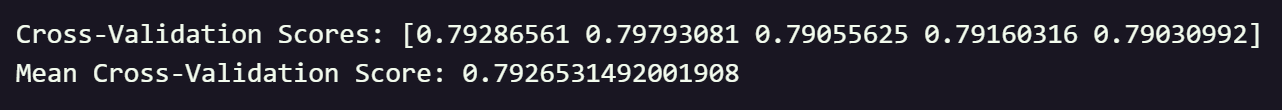
\includegraphics[width=0.6\textwidth]{media/logistic_reg_cross_val_results.png} 
        \end{figure}
    \item \textbf{Predictions: } Predictions were made on the scaled test set, and probabilities were calculated for class membership. A threshold of 0.3 was used to adjust the predicted probabilities to determine class labels.
    \item \textbf{Model Evaluation: } The model was evaluated using the confusion matrix, classification report, which included metrics such as precicion, recall, and F1-score.
        \begin{figure}[h] 
            \centering 
            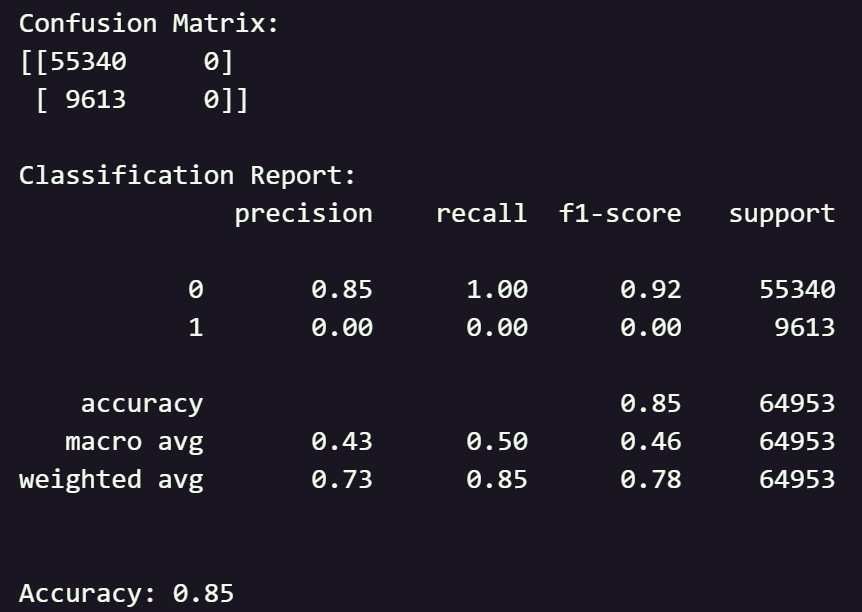
\includegraphics[width=0.35\textwidth]{media/logistic_reg_results.png} 
        \end{figure}
        \\
        \textbf{Confusion Matrix: }
        \begin{itemize}
            \item True Negatives (TN): 55,340 - The model correctly predicted that 55,340 songs are not popular (class 0).
            \item False Negatives (FN): 9,613 - The model incorrectly predicted that 9,613 popular songs (class 1) are not popular.
            \item True Positives (TP): 0 - The model did not correctly identify any songs as popular.
            \item False Positives (FP): 0 - The model did not incorrectly predict any songs as popular.
        \end{itemize}
        
        \textbf{Classification Report: }
        \begin{itemize}
            \item Precision: 
                \begin{itemize}
                    \item Class 0 (not popular): 0.85 - Among the predicted non-popular songs, 85\% were correctly identified.
                    \item Class 1 (popular): 0.0 - The model did not correctly identify any popular songs, resulting in a precision of 0.
                \end{itemize}
            \item Recall:
                \begin{itemize}
                    \item Class 0 (not popular): 1.00 - The model perfectly identified all non-popular songs (no false negatives).
                    \item Class 1 (popular): 0.0 - The model failed to identify any popular songs (no true positives).

                \end{itemize}
            \item F1-Score:
                \begin{itemize}
                    \item Class 0 (not popular): 0.92 - A high F1-score indicates a good balance between precision and recall for non-popular songs.
                    \item Class 1 (popular): 0.0 - Since there are no true positives, the F1-score is also 0.
                \end{itemize}
        \end{itemize}
        \textbf{Overall Acuracy: } 
        \\
        0.85 - The overall accuracy of the model is 85\%. However, this number is misleading in the context of a highly imbalanced dataset, as it reflects the model's ability to predict the majority class (not popular) rather than its performance on both classes.
    \item \textbf{Feature Importance: } The feature importance of the model was determined by examining the coefficients of the logistic regression model. Both feature importance for whole dataset and feature importance for each specific region has been applied. As a result of this dominant features to determine populartiy of the songs were found.
        \begin{figure}[h] 
            \centering 
            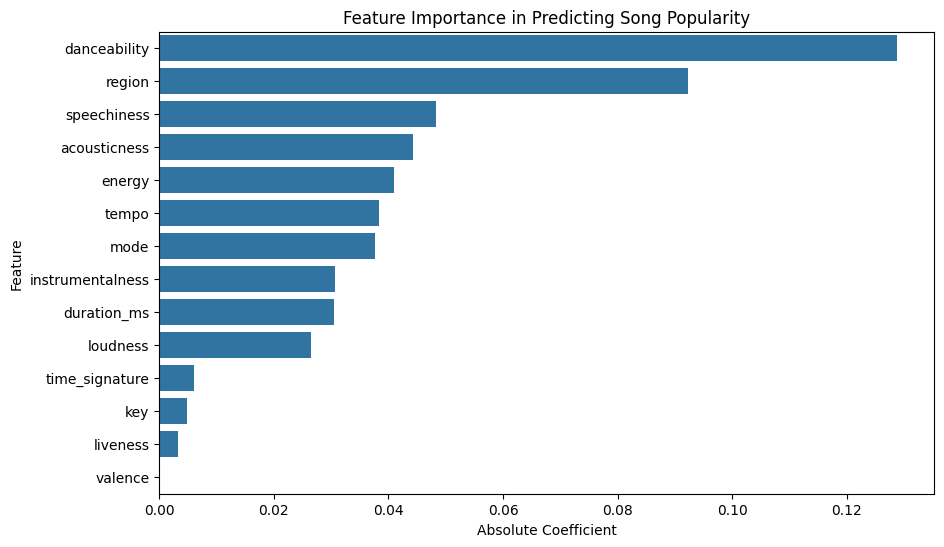
\includegraphics[width=0.7\textwidth]{media/logistic_reg_feature_imp.png} 
        \end{figure}
        \textbf{Feature Importance for Regions Examples: }
        \begin{figure}[h] 
            \centering 
            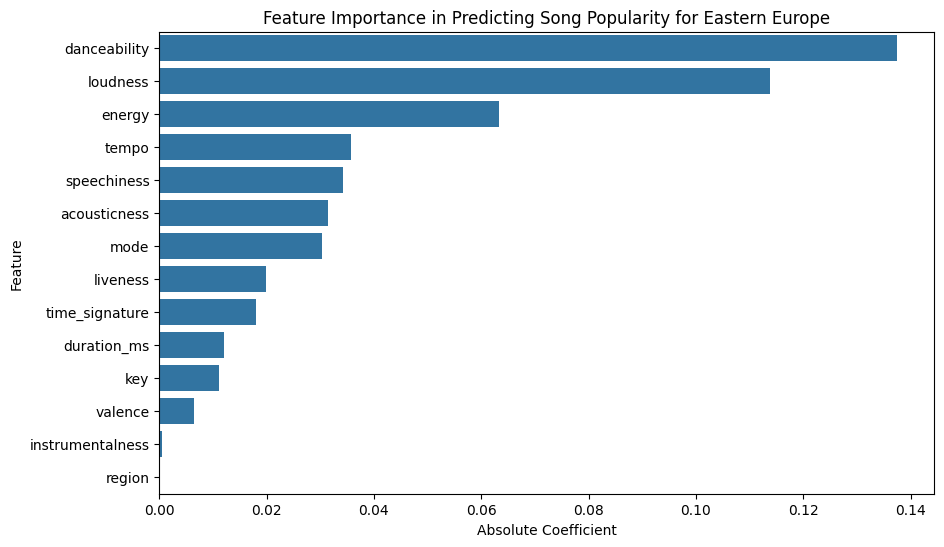
\includegraphics[width=0.7\textwidth]{media/log_reg_feature_selection_eastern_europe.png} 
        \end{figure}
        \begin{figure}[h] 
            \centering 
            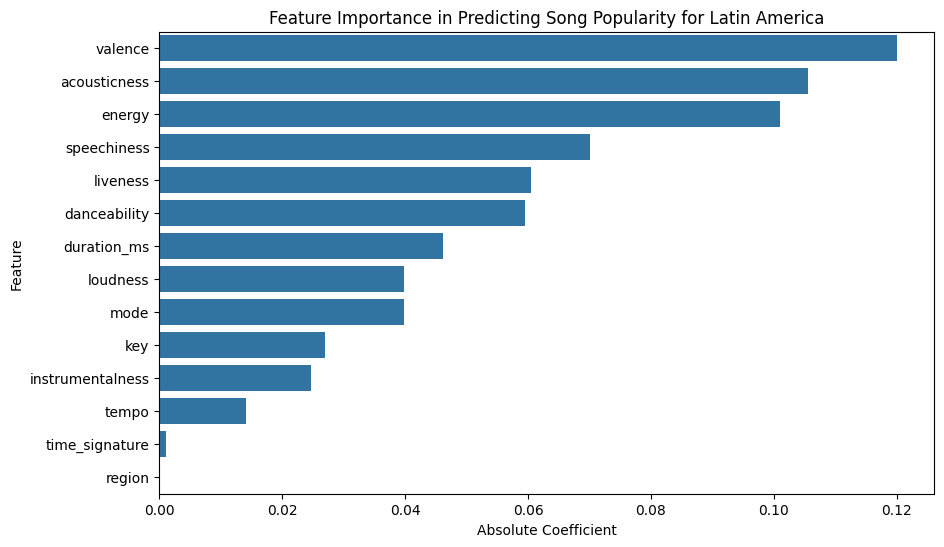
\includegraphics[width=0.7\textwidth]{media/log_reg_feature_selection_latin_america.png} 
        \end{figure}
    \item \textbf{Regional Analysis: } Regional analysis was performed to better understand how different audio features contribute to song populartiy across various regions.
        % \begin{table}[ht]
        %     \centering
        %     \begin{adjustbox}{width=\textwidth}
        %     \begin{tabular}{lrrrrrrrrrrrrrrrr}
        %     \toprule
        %     Region & Rank\_Mean & Frequency & Danceability & Energy & Key & Loudness & Mode & Speechiness & Acousticness & Instrumentalness & Liveness & Valence & Tempo & Duration\_ms & Time\_Signature & Popular \\
        %     \midrule
        %     0  & 77.28 & 51.34 & 0.686 & 0.620 & 5.21 & -7.61 & 0.507 & 0.138 & 0.259 & 0.042 & 0.168 & 0.484 & 120.41 & 219551.52 & 3.96 & 0.157 \\
        %     1  & 76.33 & 49.11 & 0.603 & 0.629 & 5.29 & -6.86 & 0.678 & 0.080 & 0.303 & 0.042 & 0.177 & 0.471 & 121.52 & 229571.73 & 3.96 & 0.117 \\
        %     2  & 69.78 & 79.65 & 0.661 & 0.641 & 5.29 & -7.34 & 0.541 & 0.130 & 0.241 & 0.056 & 0.182 & 0.471 & 122.33 & 205515.98 & 3.96 & 0.181 \\
        %     3  & 71.24 & 188.65 & 0.663 & 0.660 & 5.36 & -6.71 & 0.593 & 0.106 & 0.286 & 0.042 & 0.194 & 0.581 & 122.61 & 217127.50 & 3.94 & 0.184 \\
        %     4  & 75.45 & 61.90 & 0.642 & 0.611 & 5.29 & -7.63 & 0.462 & 0.105 & 0.295 & 0.057 & 0.178 & 0.470 & 120.14 & 213894.57 & 3.95 & 0.152 \\
        %     5  & 79.72 & 49.95 & 0.658 & 0.620 & 5.19 & -6.99 & 0.610 & 0.131 & 0.237 & 0.031 & 0.179 & 0.464 & 121.36 & 206987.98 & 3.95 & 0.127 \\
        %     6  & 78.48 & 50.92 & 0.642 & 0.636 & 5.32 & -7.35 & 0.563 & 0.109 & 0.232 & 0.044 & 0.182 & 0.486 & 121.29 & 203514.75 & 3.95 & 0.120 \\
        %     7  & 67.06 & 61.44 & 0.647 & 0.631 & 5.22 & -7.05 & 0.608 & 0.116 & 0.231 & 0.048 & 0.179 & 0.472 & 120.82 & 213396.98 & 3.96 & 0.163 \\
        %     8  & 71.30 & 98.99 & 0.623 & 0.584 & 5.24 & -7.39 & 0.659 & 0.082 & 0.359 & 0.035 & 0.172 & 0.460 & 119.92 & 222230.31 & 3.94 & 0.197 \\
        %     9  & 71.92 & 52.77 & 0.649 & 0.646 & 5.31 & -7.02 & 0.564 & 0.119 & 0.265 & 0.041 & 0.177 & 0.496 & 121.24 & 210862.34 & 3.95 & 0.125 \\
        %     10 & 81.34 & 64.66 & 0.669 & 0.643 & 5.34 & -7.26 & 0.525 & 0.145 & 0.252 & 0.056 & 0.173 & 0.489 & 120.90 & 205864.40 & 3.96 & 0.117 \\
        %     \bottomrule
        %     \end{tabular}
        %     \end{adjustbox}
        %     \end{table}
\end{itemize} 







\section{Decision Tree}




\section{Random Forest}
Random Forest is an ensemble learning method that constructs a multitude of decision trees during
training and outputs the mode of the classes as the prediction of the individual trees. Random Forest
is a versatile machine learning algorithm that can be used for both classification and regression
tasks. It is based on the concept of bagging, which involves training multiple models on different
subsets of the data and combining their predictions to improve the overall performance. Random Forest
is known for its robustness, scalability, and ability to handle high-dimensional data with ease.
In this project, Random Forest was used to predict whether the song will be popular or not based on their audio
features and release region. \\




\section{Naive Bayes}
Naive Bayes is a family of probabilistic algorithms based on Bayes' Theorem, which is used for classification tasks.
The algorithm is particularly popular for its simplicity, efficiency, and effectiveness in dealing with large datasets.
It is called "naive" because it makes the assumption that the features are independent of each other given the class label.
In this project Gaussian Naive Bayes is used to predict whether a song will be popular or not based on its audio features and release region by assuming that
the features follow a normal distribution. The fundamental principle of the Naive Bayes algorithm is Bayes' Theorem, which is expressed as:

\[
P(C | X) = \frac{P(X | C) \cdot P(C)}{P(X)}
\]

Where:
\begin{itemize}
    \item \( P(C | X) \) is the posterior probability of class \( C \) given the features \( X \).
    \item \( P(X | C) \) is the likelihood of observing the features \( X \) given class \( C \).
    \item \( P(C) \) is the prior probability of class \( C \).
    \item \( P(X) \) is the prior probability of observing the features \( X \).
\end{itemize}

To make predictions, Naive Bayes calculates the posterior probability for each class and selects the class with the highest probability. The independence assumption simplifies the calculation of the likelihood:

\[
P(X | C) = P(X_1 | C) \cdot P(X_2 | C) \cdots P(X_n | C)
\]

Where \( X_1, X_2, \ldots, X_n \) are the features.






\section{SVM}